\documentclass[landscape,twocolumn,a4paper,12pt,french]{article}

\usepackage[TD]{../../Style}

\pagestyle{empty}

\setlength{\columnsep}{2cm}

\setstretch{1.3}

% Début du document
%%%%%%%%%%%%%%%%%%%
\begin{document}

\begin{correction}[83 p154]

Soit $f:x \mapsto {\color{DarkRed}-7,5x^2}+{\color{DarkBlue}12x}$.

\strut Pour $x \in \R$, on a
$\begin{array}[t]{r>{\color{DarkRed}}cc>{\color{DarkBlue}}c}
f'(x)=&-7,5 \times 2x &+& 12 \times 1 \\
= & -15x & + & 12 \\
= & ax & + & b \\
\end{array}$

avec ${\color{DarkRed}a=-15}$ et ${\color{DarkBlue}b=12}$. Alors:

\begin{itemize}
\item Comme $a$ est négatif, le signe de $f'$ est positif puis négatif: $+ \ \ -$
\item Le \emph{zéro} de $f'$ est atteint lorsque $x=\frac {-b} {a}=\frac{-12}{-15}=\frac 4 5 = 0,8$. (On peut aussi résoudre l'équation $-15x+12=0$ dont la solution est $0,8$)
\end{itemize}

On peut donc dresser le tableau de signes de $f'$, puis en déduire le tableau de variations de $f$:

\compo
{
Enfin, on a $f(0,8) = -7,5 \times (0,8)^2 + 12 \times 0,8 = 4,8$, ce qui permet de compléter le tableau.
}
{
\begin{center}
\begin{tikzpicture}
\tkzTabInit[lgt=1.5,espcl=1.8]{$x$ /1, $f'(x)$/1, $f(x)$/2}{$- \infty$, $0.8$, $+ \infty$}
\tkzTabLine{,+,z,-}
\tkzTabVar{-/$ $, +/$4.8$, -/$ $}
\end{tikzpicture}
\end{center}
}

\strut Ce tableau nous indique alors que $f$ admet un maximum: Il s'agit de $4,8$, atteint en $0,8$.

\compo[0.6]
{
\begin{rmq}
On peut tracer la courbe de $f$ sur la calculatrice pour vérifier que le tableau obtenu est correct:
\end{rmq}
}
{
\begin{tikzpicture}
\begin{axis}[
styleglobal,
width=0.9*\linewidth,
xmin=-2, xmax=4,
ymin=-2, ymax=6,
xtick distance=1,
ytick distance=1,
]
\addplot[styleplot,domain=(-4:4)]{(-7.5*x^2+12*x} node[pos=0.55,below right]{$\mathscr C_f$};;
\end{axis}
\end{tikzpicture}
}

\end{correction}

\newpage

\begin{correction}[83 p154]

Soit $f:x \mapsto {\color{DarkRed}-7,5x^2}+{\color{DarkBlue}12x}$.

\strut Pour $x \in \R$, on a
$\begin{array}[t]{r>{\color{DarkRed}}cc>{\color{DarkBlue}}c}
f'(x)=&-7,5 \times 2x &+& 12 \times 1 \\
= & -15x & + & 12 \\
= & ax & + & b \\
\end{array}$

avec ${\color{DarkRed}a=-15}$ et ${\color{DarkBlue}b=12}$. Alors:

\begin{itemize}
\item Comme $a$ est négatif, le signe de $f'$ est positif puis négatif: $+ \ \ -$
\item Le \emph{zéro} de $f'$ est atteint lorsque $x=\frac {-b} {a}=\frac{-12}{-15}=\frac 4 5 = 0,8$. (On peut aussi résoudre l'équation $-15x+12=0$ dont la solution est $0,8$)
\end{itemize}

On peut donc dresser le tableau de signes de $f'$, puis en déduire le tableau de variations de $f$:

\compo
{
Enfin, on a $f(0,8) = -7,5 \times (0,8)^2 + 12 \times 0,8 = 4,8$, ce qui permet de compléter le tableau.
}
{
\begin{center}
\begin{tikzpicture}
\tkzTabInit[lgt=1.5,espcl=1.8]{$x$ /1, $f'(x)$/1, $f(x)$/2}{$- \infty$, $0.8$, $+ \infty$}
\tkzTabLine{,+,z,-}
\tkzTabVar{-/$ $, +/$4.8$, -/$ $}
\end{tikzpicture}
\end{center}
}

\strut Ce tableau nous indique alors que $f$ admet un maximum: Il s'agit de $4,8$, atteint en $0,8$.

\compo[0.6]
{
\begin{rmq}
On peut tracer la courbe de $f$ sur la calculatrice pour vérifier que le tableau obtenu est correct:
\end{rmq}
}
{
\begin{tikzpicture}
\begin{axis}[
styleglobal,
width=0.9*\linewidth,
xmin=-2, xmax=4,
ymin=-2, ymax=6,
xtick distance=1,
ytick distance=1,
]
\addplot[styleplot,domain=(-4:4)]{(-7.5*x^2+12*x} node[pos=0.55,below right]{$\mathscr C_f$};;
\end{axis}
\end{tikzpicture}
}

\end{correction}


\end{document}
